\documentclass[titlepage,11pt]{article}
\usepackage{comment}
\usepackage{enumitem}
\usepackage{transparent} % Untuk transparansi gambar
\usepackage{listings}
\usepackage{amsmath}
\usepackage{graphicx}
\usepackage[font=small,labelfont=bf]{caption}
\usepackage[indonesian]{babel}
\usepackage{float}
\usepackage{verbatim}
\usepackage{graphicx,tabularx,multirow}
\usepackage{xcolor}
\usepackage[onehalfspacing]{setspace}
\usepackage[
	allcolors=visigrey,
	colorlinks=true,
]{hyperref}
\usepackage[a4paper,left=2cm,right=2cm]{geometry}
% Pengaturan kutipan artikel
\usepackage[style=ieee, backend=biber]{biblatex}
%Code listing style pak akok
\definecolor{codegreen}{rgb}{0,0.6,0}
\definecolor{codegray}{rgb}{0.5,0.5,0.5}
\definecolor{codepurple}{rgb}{0.58,0,0.82}
\definecolor{backcolour}{rgb}{0.95,0.95,0.92}

\usepackage{eso-pic} % Untuk menambahkan elemen ke seluruh halaman

\newcommand\BackgroundPic{
  \put(0,0){
    \parbox[b][\paperheight]{\paperwidth}{
      \vfill
      \centering
      \transparent{0.1}
      \includegraphics[width=0.4\paperwidth,keepaspectratio]{miot.png}
      \vfill
    }
  }
}

\newcommand\BackgroundAllPages{ \AddToShipoutPicture*{\BackgroundPic} }
\newcommand\BackgroundNone{ \ClearShipoutPicture } % hilangkan background

\lstdefinestyle{mystyle}{
	backgroundcolor=\color{backcolour}, commentstyle=\color{codegreen},
	keywordstyle=\color{magenta},
	numberstyle=\small\color{codegray},
	stringstyle=\color{codepurple},
	basicstyle=\ttfamily\footnotesize,
	breakatwhitespace=false,         
	breaklines=true,                 
	captionpos=t,                    
	keepspaces=true,                 
	numbers=left,                    
	numbersep=5pt,                  
	showspaces=false,                
	showstringspaces=false,
	showtabs=false,           
	frame = single,
	tabsize=2
}
\lstset{style=mystyle}

\definecolor{visigrey}{rgb}{.1,.15,.15}
\geometry{top=1cm,bottom=.5cm}
\savegeometry{titlepage}
\geometry{top=2cm,bottom=2cm}
\savegeometry{main}

\def\bspace{\(\qquad\qquad\qquad\)}
\usepackage[T1]{fontenc}
\usepackage[utf8]{inputenc}
\usepackage{tgheros}
\renewcommand*\familydefault{\sfdefault}

\setcounter{tocdepth}{6}

\def\autor{Laboratorium }
\def\lab{Multimedia dan Internet of Things}
\def\departemen{Departemen Teknik Komputer}
\def\institut{Institut Teknologi Sepuluh Nopember}
\def\praktikum{Laporan Sementara \\ Praktikum Jaringan Komputer}
\def\nama{Moh. Wildan Risqi Maulidi - 5024231056}
% Ubah Judul sesuai dengan modul
\def\judul{Routing & Manajemen IPv6}
\def\tanggal{2025}
\begin{document}
% Ubah Bahasa sesuai dengan keinginan
\selectlanguage{indonesian}

\BackgroundNone
\def\headingtype{\bf \small}
\loadgeometry{titlepage}

\begin{titlepage}
	\centering
	\begin{tabularx}{\textwidth}{l@{\hskip 0pt}lX}
		\raisebox{-0.5\height}{
\includegraphics[width=3cm]{Cover/img/logodepart.png}} 
		& \raisebox{-0.5\height}{\includegraphics[width=3cm]{Cover/img/miot.png}} 
		& \raggedleft
	\hfill
	\begin{minipage}{0.5\textwidth}
		\raggedleft
		{\emph{\headingtype \autor}} \\[-2pt]
		{\headingtype \lab} \\[-2pt]
		{\headingtype \departemen} \\[-2pt]
		{\headingtype \emph{\institut}}
	\end{minipage}

	\vspace{5cm}
	\end{tabularx}
	
	\vspace{5cm}
	{\Huge \bf \praktikum \par}
	
	\vspace{2cm}
	{\LARGE \bf \judul \par}
	
	\vspace{2cm}
	{\Large \nama \par}
	
	\vfill
	{\Large \tanggal \par}
	
	\vfill
	
\includegraphics[width=\textwidth]{Cover/img/footer.png}
\end{titlepage}

\loadgeometry{main}


\BackgroundAllPages
% Pilih Modul yang akan di build
\section{Pendahuluan}
\subsection{Latar Belakang}
praktikum dilakukan untuk pengenalan tentang IPv6, serta mengetahui cara routing IPv6 dengan baik dan benar baik routing statis dan routing dinamis. dengan banyaknya perangkat membutuhkan internet jadinya IPv6 dibuat karena kapasitasnya sangat besar dan tidak terbatas. IPv6 juga memiliki banyak fitur yang lebih baik dibandingkan IPv4, seperti keamanan yang lebih baik, pengalamatan yang lebih efisien, dan dukungan untuk mobilitas perangkat.\\

\subsection{Dasar Teori}
%Bagian ini memuat teori-teori dasar yang mendukung pelaksanaan praktikum. Penjelasan mencakup konsep teknis, nama istilah, serta prinsip ilmiah yang relevan. Tujuannya adalah untuk memberikan pemahaman mendalam sebelum praktikum dilakukan.%
\subsection*{IPv6 (Internet Protocol Version 6)}

IPv6 adalah versi terbaru dari protokol Internet yang menggantikan IPv4. IPv6 menggunakan panjang alamat 128-bit, yang memungkinkan ketersediaan lebih dari $3.4 \times 10^{38}$ alamat unik, dibandingkan IPv4 yang hanya mendukung sekitar 4.3 miliar alamat. Pengembangan IPv6 didorong oleh keterbatasan alamat pada IPv4, serta kebutuhan akan konektivitas global yang lebih besar, termasuk untuk perangkat Internet of Things (IoT). Selain itu, IPv6 menyediakan fitur-fitur seperti autokonfigurasi, keamanan end-to-end, dan efisiensi routing yang lebih baik.

\subsection*{Subnetting pada IPv6}

Subnetting pada IPv6 dilakukan dengan menggunakan \textit{prefix} untuk menunjukkan ukuran jaringan. Sebagai contoh, prefix \texttt{/32} berarti 32 bit pertama digunakan sebagai penanda network ID. Umumnya, subnet pada IPv6 dibuat menggunakan prefix \texttt{/64}. Contoh pembentukan subnet:
\begin{itemize}
    \item \texttt{2001:db8:0000:0000::/64}
    \item \texttt{2001:db8:0001:0000::/64}
    \item \texttt{2001:db8:0002:0000::/64}
\end{itemize}
Subnetting ini mempermudah pengelolaan jaringan besar dan memberikan struktur alamat yang lebih fleksibel.

\subsection*{Routing IPv6}

Routing pada IPv6 dapat dilakukan secara statis maupun dinamis:
\begin{itemize}
    \item \textbf{Routing Statis:} Administrator jaringan secara manual menentukan rute antar jaringan. Cocok digunakan pada jaringan kecil dan konfigurasi sederhana.
    \item \textbf{Routing Dinamis:} Protokol routing seperti OSPFv3, RIPng, dan BGP digunakan agar router dapat saling bertukar informasi rute secara otomatis. Cocok untuk jaringan yang besar dan kompleks.
\end{itemize}
IPv6 juga menyederhanakan header paket untuk mendukung efisiensi dalam proses routing.

\subsection*{Manfaat IPv6}

IPv6 memiliki sejumlah keunggulan dibandingkan IPv4, antara lain:
\begin{itemize}
    \item Tidak memerlukan NAT (Network Address Translation), sehingga komunikasi end-to-end lebih langsung dan efisien.
    \item Mendukung autokonfigurasi alamat menggunakan Stateless Address Autoconfiguration (SLAAC).
    \item Mendukung keamanan data melalui penerapan IPsec yang terintegrasi secara default.
    \item Efisiensi dalam routing karena struktur alamat yang hierarkis dan penggunaan header yang sederhana.
\end{itemize}

%===========================================================%
\section{Tugas Pendahuluan}
Bagian ini berisi jawaban dari tugas pendahuluan yang telah anda kerjakan, beserta penjelasan dari jawaban tersebut
\begin{enumerate}
	\item IPv6 adalah versi terbaru dari protokol internet (IP) yang dirancang untuk menggantikan IPv4. IPv6 memiliki ruang alamat yang jauh lebih besar (128 bit), memungkinkan untuk mendukung jumlah perangkat yang jauh lebih besar yang terhubung ke internet.\\
	perbedaan utama dari IPv6 dengan IPv4 sebagai berikut:\\
	\begin{table}[h!]
		\centering
		\begin{tabular}{|l|l|l|}
		\hline
		\textbf{Aspek} & \textbf{IPv6} & \textbf{IPv4} \\ \hline
		Panjang Alamat                  & 128-bit (heksadesimal)                      & 32-bit (desimal)                    \\ \hline
		Penulisan                       & Hexadecimal, dipisahkan titik dua (::)      & Desimal, dipisahkan titik (.)       \\ \hline
		NAT                             & Tidak diperlukan (alamat publik langsung)   & Umumnya menggunakan NAT             \\ \hline
		Konfigurasi                     & SLAAC, DHCPv6                               & DHCP, konfigurasi manual            \\ \hline
		Header                          & Tetap 40 byte, tanpa checksum               & Ukuran variabel, dengan checksum    \\ \hline
		\end{tabular}
	\end{table}

	\item a. Blok \textbf{\textit{2001:db8::/32}}	memiliki 32 bit prefix. Untuk membuat subnet /64, kita perlu menambahkan 32 bit lagi.\\
	b.\\
	\begin{table}[h!]
		\centering
		\begin{tabular}{|l|l|}
		\hline
		\textbf{Subnet} & \textbf{Alamat Prefix IPv6} \\ \hline
		Subnet A & \textbf{\textit{2001:db8:0:1::/64}}\\ \hline
		Subnet B & \textbf{\textit{2001:db8:0:2::/64}} \\ \hline
		Subnet C & \textbf{\textit{2001:db8:0:3::/64}} \\ \hline
		Subnet D & \textbf{\textit{2001:db8:0:4::/64}} \\ \hline
		\end{tabular}
	\end{table}
	\\\\\\
	
	\item a. lihat pada tabel dibawah:\\
	\begin{table}[h!]
		\centering
		\begin{tabular}{|l|l|l|}
		\hline
		\textbf{Subnet} & \textbf{Alamat Prefix IPv6} \\ \hline
		ether1 & Subnet A & \textbf{\textit{2001:db8:0:1::/64}}\\ \hline
		ether2 & Subnet B & \textbf{\textit{2001:db8:0:2::/64}} \\ \hline
		ether3 & Subnet C & \textbf{\textit{2001:db8:0:3::/64}} \\ \hline
		ether4 & Subnet D & \textbf{\textit{2001:db8:0:4::/64}} \\ \hline
		\end{tabular}
	\end{table}

	b.Konfigurasi IPv6 address (contoh di MikroTik CLI)\\
	\begin{lstlisting}[style=bashstyle]
	/ipv6 address
	add address=2001:db8:0:1::1/64 interface=ether1
	add address=2001:db8:0:2::1/64 interface=ether2
	add address=2001:db8:0:3::1/64 interface=ether3
	add address=2001:db8:0:4::1/64 interface=ether4
	\end{lstlisting}

	\item \begin{lstlisting}
		/ipv6 route
		add dst-address=2001:db8:0:2::/64 gateway=2001:db8:0:2::1
		add dst-address=2001:db8:0:3::/64 gateway=2001:db8:0:3::1
		add dst-address=2001:db8:0:4::/64 gateway=2001:db8:0:4::1
		add dst-address=2001:db8:0:1::/64 gateway=2001:db8:0:1::1
	\end{lstlisting}

	\item \textbf{Routing statis} adalah metode penentuan jalur jaringan secara manual oleh administrator jaringan. Jalur atau rute ditentukan secara eksplisit tanpa menggunakan protokol routing dinamis.\\
	\textbf{Fungsi Routing Statis IPv6:}\\
	\begin{itemize}
		\item Mengontrol lalu lintas jaringan secara presisi.
		\item Menghindari kompleksitas protokol dinamis.
		\item Cocok untuk jaringan kecil atau topologi tetap.
	\end{itemize}\\
	\textbf{Kapan digunakan?}\\
	\begin{itemize}
		\item Jaringan kecil dengan sedikit perubahan.
		\item Topologi sederhana.
		\item Untuk menghindari overhead protokol dinamis.
		\item Saat troubleshooting jaringan.
		\item Ketika ingin lock route ke satu jalur saja (misal untuk alasan keamanan).
	\end{itemize}
\end{enumerate}

\end{document}